\begin{pastexam}[label={px:gw3-100-ds-02}]{關務三等資訊處理 100 年 第二題}
（申論；25 分）

下圖為 min heap，請回答下列問題：（25 分）
\begin{center}
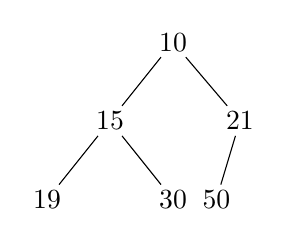
\begin{tikzpicture}[x=1cm,y=1cm,every node/.style={inner sep=2pt}]
\node (10) at (1.6,0) {10};
\node (15) at (0.8,-1.0) {15};
\node (21) at (2.45,-1.0) {21};
\node (19) at (0,-2.0) {19};
\node (30) at (1.6,-2.0) {30};
\node (50) at (2.15,-2.0) {50};
\draw (10)--(15); \draw (10)--(21); \draw (15)--(19); \draw (15)--(30); \draw (21)--(50);
\end{tikzpicture}
\end{center}
\begin{itemize}[leftmargin=2.2em]
\item[㈠] 畫出 min heap 實際上在大小為 10 的 array 中的 data structure。
\item[㈡] insert 11 至 min heap 之後，

\quad 1.畫出 insert 後的 tree-like min heap。

\quad 2.畫出其 array data structure。
\item[㈢] 承上，再 delete root 且向 left sub-tree 調整，

\quad 1.畫出調整後的 tree-like min heap。

\quad 2.畫出其 array data structure。
\end{itemize}
\end{pastexam}

\begin{pastsoln}
堆積的陣列表示、插入（往上調整）和刪除根（往下調整）見資結書第~8.1~節。 陣列用索引 $1$ 開始的慣例：大小 $10$ 的陣列索引 $0..9$，$A[0]$
不用，根在 $A[1]$，$A[i]$ 的子節點在 $A[2i]$、$A[2i+1]$，父節點在 $A[\lfloor i/2 \rfloor]$。 （若用索引 $0$ 開始，子節點是 $2i+1$、$2i+2$，
下面每個陣列整體往左移一格即可，內容順序相同。）

\textbf{㈠}。 依層序（由上而下、由左而右）放入：
\begin{center}
\small
\begin{tabular}{l|*{10}{c|}}
\cline{2-11}
索引 & 0 & 1 & 2 & 3 & 4 & 5 & 6 & 7 & 8 & 9 \\ \cline{2-11}
$A$ & — & 10 & 15 & 21 & 19 & 30 & 50 & & & \\ \cline{2-11}
\end{tabular}
\end{center}
$n = 6$。 檢查：$A[3] = 21$ 只有左子 $A[6] = 50$，和圖上 50 掛在 21 下面一致。

\textbf{㈡ 插入 11}。 先放到最後一格 $A[7]$（21 的右子），再往上調整：
\begin{itemize}
\item $A[7] = 11$，父節點 $A[3] = 21 > 11$，交換：$A[3] = 11$、$A[7] = 21$。
\item $A[3] = 11$，父節點 $A[1] = 10 \le 11$，停止。
\end{itemize}
\begin{center}
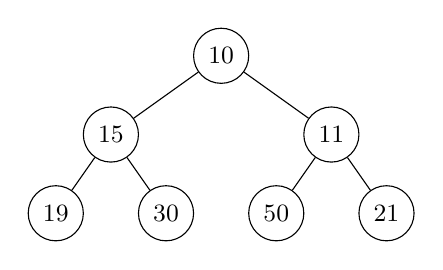
\begin{tikzpicture}[level distance=10mm,level 1/.style={sibling distance=28mm},level 2/.style={sibling distance=14mm},
  every node/.style={circle,draw,minimum size=7mm,inner sep=0pt,font=\small}]
\node {10}
  child {node {15} child {node {19}} child {node {30}}}
  child {node {11} child {node {50}} child {node {21}}};
\end{tikzpicture}
\qquad
\begin{tabular}[b]{l|*{10}{c|}}
\cline{2-11}
索引 & 0 & 1 & 2 & 3 & 4 & 5 & 6 & 7 & 8 & 9 \\ \cline{2-11}
$A$ & — & 10 & 15 & 11 & 19 & 30 & 50 & 21 & & \\ \cline{2-11}
\end{tabular}
\end{center}

\textbf{㈢ 刪除根}。 題目的「向 left sub-tree 調整」不是標準說法。 min heap 刪除根的標準做法是：取出根 10，把最後一個元素 $A[7] = 21$ 搬到根，
$n$ 變成 $6$，再往下調整，每一步和\textbf{較小}的子節點交換；往哪一邊走由兩個子節點誰小決定，不能自己指定。 這裡根的兩個子節點是
15（左）和 11（右），只能和 11 交換，若硬把左子樹的 15 換上來當根，$15 > 11$ 就違反 min heap。 下面照標準做法：
\begin{itemize}
\item 取出 10，$A[1] \gets 21$，$A[7]$ 清空。
\item $A[1] = 21$，子節點 $A[2] = 15$、$A[3] = 11$，較小的是 11，$21 > 11$，交換：$A[1] = 11$、$A[3] = 21$。
\item $A[3] = 21$，子節點只剩 $A[6] = 50$，$21 \le 50$，停止。
\end{itemize}
\begin{center}
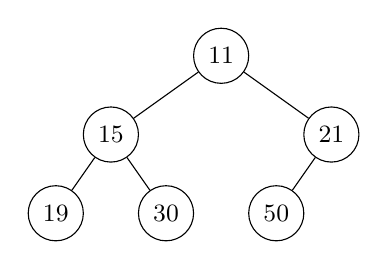
\begin{tikzpicture}[level distance=10mm,level 1/.style={sibling distance=28mm},level 2/.style={sibling distance=14mm},
  every node/.style={circle,draw,minimum size=7mm,inner sep=0pt,font=\small}]
\node {11}
  child {node {15} child {node {19}} child {node {30}}}
  child {node {21} child {node {50}} child[missing]};
\end{tikzpicture}
\qquad
\begin{tabular}[b]{l|*{10}{c|}}
\cline{2-11}
索引 & 0 & 1 & 2 & 3 & 4 & 5 & 6 & 7 & 8 & 9 \\ \cline{2-11}
$A$ & — & 11 & 15 & 21 & 19 & 30 & 50 & & & \\ \cline{2-11}
\end{tabular}
\end{center}
調整後根是新的最小值 11，左子樹 $\{15, 19, 30\}$ 完全沒動。 插入和刪除各 $O(\log n)$。
\end{pastsoln}
